\section{The \emph{k}-means problem}
The $k$-means optimization problem is defined as:
\begin{enumerate}
\item \underline{Input}: A set of $n$ points $x_1,....x_n \in
\mathbb{R^d}$ and a positive integer $k<n$.
\item \underline{Output}: $T \subset  \mathbb{R^d}$ s.t. $|T|=k$. 
\item \underline{Goal}: minimize "cost" of $T$ where: $cost(T) 
:= \sum_{i = 1}^{n} \min_{\mu_j \in T} \norm{x_i-\mu_j}^2 $.
\end{enumerate}

As before, we can attempt and exhaustive search with exponential
time complexity. If we want some solution in polynomial time, we
must settle for an approximation, as $k$-means is also an NP-hard
optimization problem. One approximate solution is Lloyd's method
for $k$-means:

\begin{algorithm}
\caption{Lloyd k-means algorithm}
\begin{algorithmic} 
\STATE Pick randomly $x_1,...,x_k $ from $\mathcal{X}$ \;
\WHILE{stopping criteria not satisfied}
\STATE Assign points of the dataset to the closest center \;
\STATE Get the clusters $C_1, ..., C_k$\;
\STATE Compute the new centroïds $\mu_j = \frac{1}{|C_j|}
\sum_{x_i\in C_j} x_i$, $\forall j \in \{1,...,k\}$\;
\ENDWHILE
\end{algorithmic}
\end{algorithm}

\begin{remark}
As $k$-means is NP hard, Lloyd's method gives us an approximate
solution. However, we cannot give any approximation guarantees
on the solution, as the approximation may be arbitrarily bad.
\end{remark}

\begin{example} Consider the following setting and dataset
where $k=2$ and $d=1$:
\begin{figure}
    \centering
    \captionsetup{width=0.8\textwidth}
    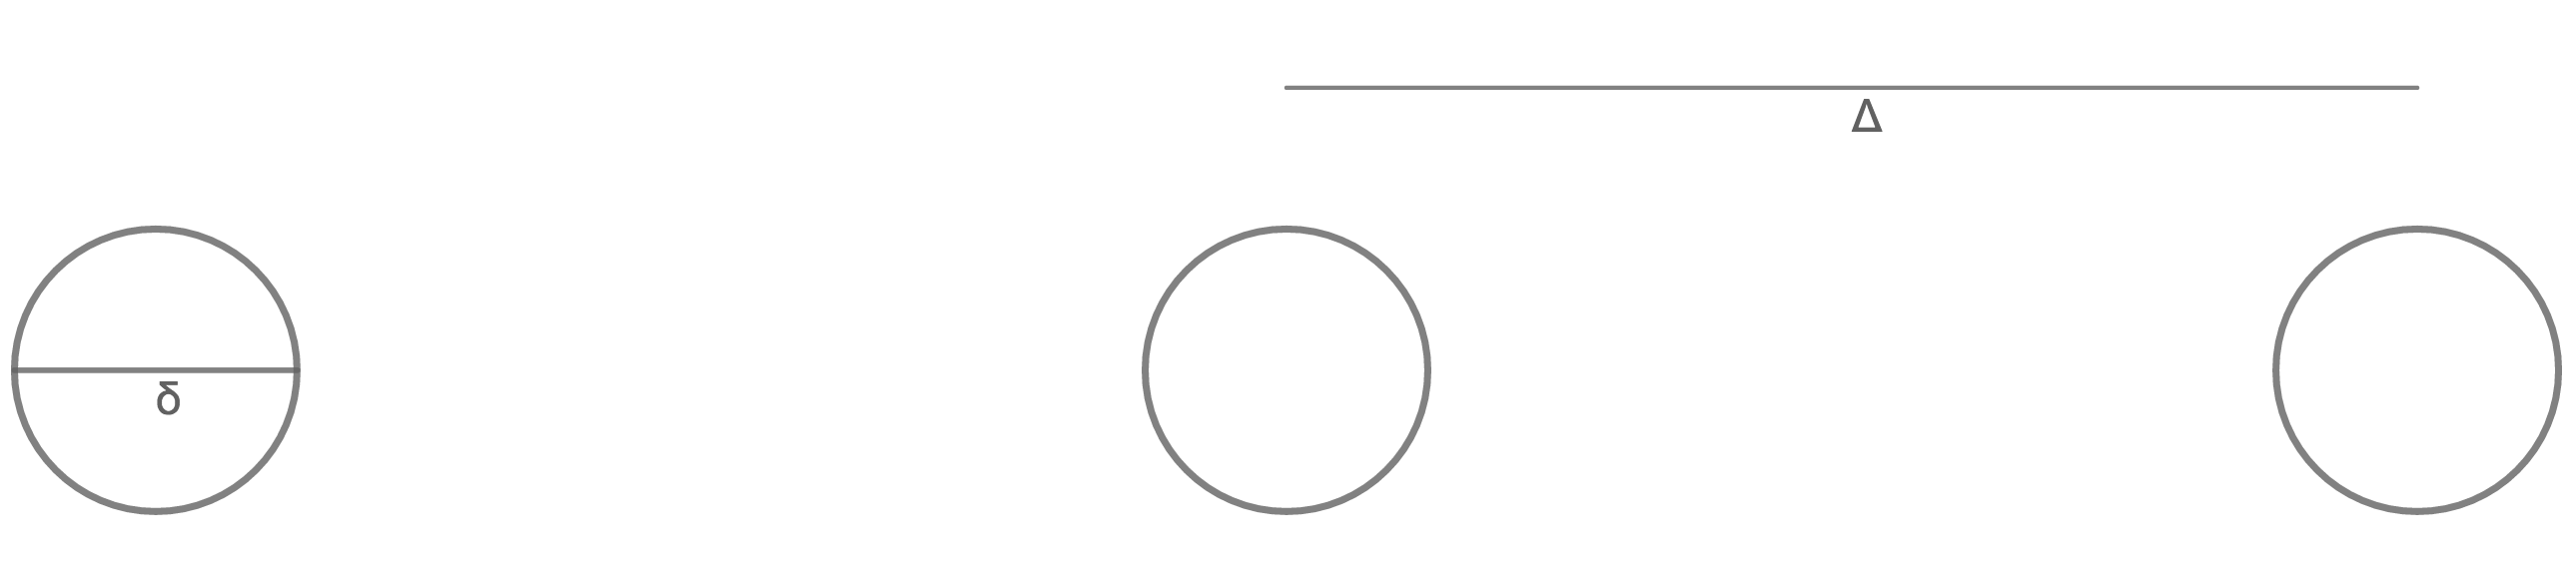
\includegraphics[scale=0.4]{chapter_1/files/kmeans.png}
    \caption{An example of datapoints and initial setting where
    Lloyd's algorithm fails to be optimal.}
    \label{fig:kmeans}
\end{figure}
The dashed lines point to the current cluster centers, with 0
for the blue cluster and 28 for the red cluster. On this
setting, Lloyd's algorithm makes no further improvement (it
terminates after one iteration), since the middle point at 16
is closer to the red cluster center 28 than to the blue cluster
center 0. And the total cost is $0^2+12^2+12^2=288$.

However, the optimal cluster center assignment should be 8 for
the blue cluster and 40 for the red cluster, which gives a cost
of $8^2+8^2+0^2=128$. Thus, Lloyd's algorithm does not give the
optimal solution.
\end{example}

\section{Further reading}
For a general reference to clustering algorithms, see \cite{har75}
or \cite{gon85}. On the hardness of $k$-means, see \cite{das2008}.
A local search approximation is given in \cite{kan2004}. The 
$k$-means++ algorithm is in \cite{art2007}.
